\documentclass[a4paper]{jpconf}

\usepackage{bm}
\usepackage{amsmath}
\usepackage{amssymb}
\usepackage{graphicx}
\usepackage{nicefrac}
\usepackage{tikz}
\usepackage{pgfplots}
\usepackage[detect-weight=true, binary-units=true]{siunitx}

\usetikzlibrary{positioning,shapes,arrows,calc,intersections}
\usepgfplotslibrary{dateplot}
\pgfplotsset{compat=1.8}

\begin{document}

\title{
  Fast divergence-conforming reduced basis methods for stationary
  and transient flow problems
}

\author{
  E Fonn$^{1}$,
  H van Brummelen$^{2}$,
  T Kvamsdal$^{1,3}$ and
  A Rasheed$^{1,4}$
}
\address{
  $^{1}$ Department of Applied Mathematics and Cybernetics, SINTEF Digital \\
  $^{2}$ Department of Mechanical Engineering, Eindhoven University of Technology \\
  $^{3}$ Department of Mathematical Sciences, Norwegian University of Science and Technology \\
  $^{4}$ Department of Engineering Cybernetics, Norwegian University of Science and Technology
}
\ead{eivind.fonn@sintef.no}

\begin{abstract}
  Reduced basis methods (RB methods or RBMs) form one of the most
  promising techniques to deliver numerical solutions of parametrized
  PDEs in real-time with reasonable accuracy \cite{Quarteroni2016rbm}.
  For the Navier-Stokes equation, RBMs based on LBB-stable
  velocity-pressure spaces do not generally inherit the stability of
  the high-fidelity method. Techniques for working around this
  problem, e.g. by inflating the reduced velocity space with so-called
  supremizer modes \cite{Ballarin2015ssp} have the effect of
  deteriorating the performance of the RBM in the performance-critical
  online stage.

  We show how a solenoidal reduced formulation arising from a
  divergence-conforming high-fidelity model eliminates this problem,
  producing RBMs that are faster by an order of magnitude or more in
  the online stage. This formulation is most easily achieved using
  divergence-conforming compatible B-spline bases mapped through Piola
  transforms under variable geometries. See \cite{Fonn2018fdc} for
  more details.

  We also demonstrate the flexibility of RBMs for non-stationary flow
  problems using a problem with two stages: an initial, finite
  transient stage where the flow pattern settles from the initial
  data, followed by a terminal and infinite oscillatory stage
  characterized by vortex shedding. We show how an RBM whose data is
  only sourced from the terminal stage nevertheless can produce
  solutions that pass through the initial stage without critical
  problems (e.g. crashing, diverging or blowing up).
\end{abstract}

\section{Introduction}

Conventional methods for simulating partial differential equations
include well-established techniques such as Finite Volume Methods
(FVM), Finite Difference Methods (FDM) and Finite Element Methods
(FEM).  Common to all of these methods is the large number of degrees
of freedom that is typically required to accurately model a physical
system, often numbering in the millions or billions. Given the good
and well-established approximation properties of FVM, FDM and in
particular FEM, such models are usually classified as
\emph{high-fidelity} models.  Problems of this size are not generally
possible to solve in practical timeframes except on specialized
hardware, and even then they may require several days of computing
time.  This prohibits the use of high-fidelity models in time-critical
on-site analyses, e.g.~for developing predictive digital
twins~\cite{Rasheed2020dtv}.

This computational complexity is also at odds with the increasing
demand for real-time low-cost models for the repetitive solution of
physical models in \emph{many-query scenarios}.  This is particularly
relevant in optimization, control systems, inverse and inference
problems and uncertainty quantification.  Common for many of these
applications is that the model in question is \emph{parametrized} by a
suitably small number of input parameters.  It is often required to be
able to provide solutions in the sub-second regime.

Reduced-order modeling (ROM) provides a paradigm to address the
aforementioned challenges.  ROM is a rapidly developing
field~\cite{Bazaz2012rpm}. The general aim of ROM is to replace the
original model with a \emph{reduced model} of very modest
computational complexity. Within this general framework of ideas, one
of the most promising is that of \emph{reduced basis methods}
(RBM). This method dates back to the 1980s with work from
\cite{Almroth1978acg,Almroth1981gfi,Nagy1979mrg,Noor1980rbt,Noor1981bpb,Noor1981rar,Noor1982mln}.
Excellent modern introductions can be found in
\cite{Quarteroni2016rbm,Haasdonk2017rbm}.

The fundamental concept of RB methods is to formulate the problem on a
function space with very low dimension, where the basis functions are
tailored to the solution of the model in the parameter regime of
interest.  In comparison, while e.g.~FEM can boast well-established
asymptotic approximation properties, the approximation power per
degree-of-freedom is clearly limited.  RB methods seek to construct a
basis with optimal approximation properties for the given class of
solutions, under the premise that the cost of constructing the basis
is inconsequential.  This premise arises because of the
\emph{offline/online} division.  The \emph{offline stage}, where the
basis is constructed, is run only once, the result of which is a RBM
which can be used in the \emph{online stage}, to be run for each
parameter query.

This paper is concerned with the application of a solenoidal RBM for
Navier-Stokes flow problems.  This method is detailed in
\cite{Fonn2018fdc} for stationary flow problems, where significant
performance improvements were found relative to a traditional RBM with
velocity, pressure and stabilizing ``supremizer'' modes, as in
\cite{Ballarin2015ssp}.  Some of the theory and results from
\cite{Fonn2018fdc} is repeated here.

Further, we aim to investigate the applicability of RBMs to
non-stationary flow problems characterized by multiple ``stages'': a
flow problem with a significant but finite ``ramp up'' stage followed
by a non-terminating flow pattern characterized by vortex shedding.
In this context we envision that the vortex shedding stage is of
primary interest, and it is therefore desirable to avoid including
degrees-of-freedom which are sourced from the ramping-up stage.  From
an approximation utility point of view, such degrees-of-freedom are
costly and not benefitial.  We will demonstrate that an RBM whose
solution space has been sourced \emph{only} from the vortex shedding
stage is able to produce a time-stepping sequence that can robustly
reach this stage.

\section{Parametrized Navier-Stokes equations}

\label{sec:setting}
We consider the non-stationary Navier-Stokes equations,
\begin{alignat}{2}
  \label{eqn:ns-1}
  \partial_t \bm u + (\bm u \cdot \nabla) \bm u - \nu \Delta \bm u + \nabla p &= \bm f && \qquad \text{in } [0,T] \times \Omega, \\
  \label{eqn:ns-2}
  \nabla \cdot \bm u &= 0 && \qquad \text{in } \Omega, \\
  \label{eqn:ns-3}
  \bm u &= \bm g && \qquad \text{on } \Gamma_\text{D}, |\Gamma_D| > 0 \\
  \label{eqn:ns-4}
  -p \bm n + \nu (\nabla \bm u) \bm n &= \bm h && \qquad \text{on } \Gamma_\text{N}, \\
  \label{eqn:ns-5}
  \bm u(t=0) &= \bm u_0 && \qquad \text{on } \Omega.
\end{alignat}
where $\nu$ is the viscosity, $\bm u, p$ are the unknown velocity and
pressure, $\bm{f},\bm{g},\bm{h},\bm{u}_0$ correspond to exogenous and
initial data, $\Omega \subset \mathbb R^d$ is the domain of interest
with boundary
$\partial \Omega = \Gamma_\text{D} \cup \Gamma_\text{N}$,
$\Gamma_\text{D} \cap \Gamma_\text{N} = \emptyset$, $\bm{n}$ denotes
the external unit normal vector, and $T$ is the upper boundary in
time.

The weak Galerkin formulation of the problem is to find $(\bm u, p)$
members of suitable function spaces, such that for all $(\bm w, q)$,
also members of suitable function spaces, it holds that
\begin{align}
  m(\dot{\bm u}, \bm w) + a(\bm u, \bm w) + c(\bm u, \bm u, \bm w) + b(p, \bm w) &= d(\bm w), \label{eqn:var-1} \\
  b(q, \bm u) &= 0, \label{eqn:var-2}
\end{align}
where the linear, bilinear and trilinear forms $m,a,b,c,d$ are defined as
\begin{subequations}
\begin{align}
  m(\bm u, \bm w) &= \int_\Omega \bm u \cdot \bm w, \label{eqn:form-m} \\
  a(\bm u, \bm w) &= \nu \int_\Omega \nabla \bm u : \nabla \bm w, \label{eqn:form-a} \\
  b(p, \bm w) &= -\int_\Omega p \nabla \cdot \bm w, \label{eqn:form-b} \\
  c(\bm u, \bm v, \bm w) &= \int_\Omega (\bm u \cdot \nabla) \bm v \cdot \bm w, \label{eqn:form-c} \\
  d(\bm w) &= \int_{\Gamma_\text{N}} \bm h \cdot \bm w + \int_{\Omega} \bm f \cdot \bm w. \label{eqn:form-d}
\end{align}
\end{subequations}
In the following it will be assumed that all function spaces involved
in this formulation are linear.  This is generally not the case,
unless $\bm g \equiv \bm 0$, but the process for transforming a
non-homogeneous model into a homogenous one by the use of a
\emph{lift function} is well known, see e.g.~\cite{Fonn2018fdc}.

We now consider the case when the problem \eqref{eqn:ns-1}--\eqref{eqn:ns-5}
depends on a number of parameters.  We will denote by $\mathcal{P}$
the parameter space, and by $\bm \mu$ any given element of $\mathcal{P}$.

The effect of varying parameters influences not only the solutions
$\bm u$ and $p$, but also the weak forms
\eqref{eqn:form-m}--\eqref{eqn:form-d} directly.  This is most
obviously the case for example with \emph{physical parameters} such as
the viscosity $\nu$ in \eqref{eqn:form-a}, \emph{data parameters} such
as $\bm g, \bm h$ (the former entering
\eqref{eqn:form-m}--\eqref{eqn:form-d} via a parameter-dependent lift
function), but one may also consider \emph{geometric parameters},
where the domain $\Omega$ itself may be transformed.

For geometric parameters, it is necessary to define a reference domain
$\hat{\Omega}$, a mapping
$\chi_{\bm \mu} : \Omega(\bm \mu) \to\hat{\Omega}$,
and function space homeomorphisms for velocity and pressure,
\begin{align}
  \label{eqn:trf-v}
  {\pi}_{\bm\mu}^\textsc{v}:& \quad [H^1(\hat{\Omega})]^d\to{}[H^1(\Omega(\bm \mu))]^d, \\
  {\pi}_{\bm\mu}^\textsc{p}:& \quad L^2(\hat{\Omega})\to{}L^2(\Omega(\bm{\mu})).
\end{align}
Thus, for example, \eqref{eqn:form-a} can be properly parametrized as
\begin{equation}
  ({\bm\pi}^*_{\bm\mu}a)\big(\hat{\bm{u}},\hat{\bm{w}};\bm{\mu}\big) =
  a\big({\pi}_{\bm\mu}^\textsc{v}\hat{\bm{u}},{\pi}_{\bm\mu}^\textsc{v}\hat{\bm{w}};\bm{\mu}\big)
\end{equation}
In this way, the entirety of \eqref{eqn:form-m}--\eqref{eqn:form-d}
can be formulated as a parameter-dependent homogeneous problem on a
fixed reference domain, involving fixed, linear function spaces for
velocity and pressure.  See \cite{Fonn2018fdc} for further details.

\section{Model order reduction}

To apply the RB method, we first solve the high-fidelity Navier-Stokes
problem for a suitably large and varied choice of parameter instances
$\bm \mu$.  The resulting ensemble is then compressed using Proper
Orthogonal Decomposition (POD) \cite{Chatterjee2000ipo} into a reduced
basis which can be represented as a tall matrix $\bm V$ of $m$
columns, where each column represents one reduced basis function.

The reduced system of equations can then be formulated. Given a
high-fidelity model represented as
\begin{equation}
  \bm A(\bm \mu) \bm u(\bm \mu) = \bm f(\bm \mu)
  \label{eqn:system}
\end{equation}
where $\bm A(\bm \mu)$ and $\bm f(\bm \mu)$ are the discrete
system matrix and right hand side arising from
\eqref{eqn:var-1}--\eqref{eqn:var-2}, we make the assumption that the
solution coefficient vector $\bm u(\bm \mu)$ can be written in
terms of the columns of $\bm V$,
\begin{equation}
  \bm u(\bm \mu) \approx \bm V \bm u_\text{r}(\bm \mu)
\end{equation}
where the vector $\vec{\bm u}_\text{r}(\bm \mu)$ is the coefficient
vector in the reduced basis. Since \eqref{eqn:system} is now
overdetermined, we can reduce the system from the left in a similar
manner, effectively forming a reduced Galerkin formulation.
\begin{equation}
  \bm V^\intercal \bm A(\bm \mu) \bm V \bm u_\text{r}(\bm \mu) = \bm V^\intercal \bm f(\bm \mu).
  \label{eqn:rsystem}
\end{equation}
For a modest number of reduced basis functions $m$, this system is
small and quickly solvable.  However, unless certain assumptions on
$\bm A$ and $\bm f$ are met, it may not be possible to quickly
assemble it.  We call this the assumption of affine representations:
that $\bm A$ and $\bm f$ can be written in the form
\begin{equation}
  \bm A(\bm \mu) = \sum_{i=1}^{M} \theta_i(\bm \mu) \bm A_i, \qquad
  \bm f(\bm \mu) = \sum_{i=1}^{N} \xi_i(\bm \mu) \bm f_i.
  \label{eqn:affine}
\end{equation}
This allows us to compute all matrices $\bm V^\intercal \bm A_i \bm V$
in the offline stage, whence
\begin{equation}
  \bm V^\intercal \bm A(\bm \mu) = \sum_{i=1}^{M} \theta_i(\bm \mu)
  \left[ \bm V^\intercal \bm A_i \bm V \right]
\end{equation}
is easily and quickly assembled in the online stage.

The assumption \eqref{eqn:affine} is not always easily realized,
especially when it comes to geometric parameters.  In many cases it
may be necessary to approximate it with various interpolation
techniques, such as the Empirical Interpolation Method (EIM)
\cite{Quarteroni2016rbm}.  For the model problems in
\cite{Fonn2018fdc} the affine representation was produced with
explicitly truncated series expansions.

\section{Solenoidal reduced basis methods}

It can be readily observed from \eqref{eqn:var-1}--\eqref{eqn:var-2}
and \eqref{eqn:form-m}--\eqref{eqn:form-d} that if the velocity
solution and test spaces are fully solenoidal (that is,
divergence-free), the expressions involving the $b$-form vanish,
and the continuity equation is trivially satisfied.  This desirable
state of affairs is not easily realized with high-fidelity methods,
because generic solenoidal function spaces are difficult to make.

Isogeometric analysis (IGA) has recently come to the forefront in this
field.  While IGA velocity basis functions are also not
\emph{in themselves} solenoidal, the method, more easily than for
classical finite element methods, allows the formulation of
divergence-conforming discretizations, which produce strongly
solenoidal solutions
\cite{Buffa2010iae, Buffa2011ias, Evans2012dsa, Evans2013idc1,
  Evans2013idc2, Evans2013idc3, Johannessen2015dcd,Opstal2017idc}.

In a classic RBM setting, each basis function is a linear combination
of weakly solenoidal high-fidelity solutions, thus also weakly
solenoidal.  If, as with IGA, the high-fidelity method can produce
strongly solenoidal solutions, the reduced basis functions will also
be strongly solenoidal, so a velocity-only reduced formulation is
possible.  The pressure solution can be recovered, if necessary, using
\emph{supremizers} \cite{Ballarin2015ssp} as a stabilizing velocity
test space.  The details for this can be found in \cite{Fonn2018fdc}.

Solenoidal RBMs can be significantly faster than conventional RBMs, as
we demonstrate in Section~\ref{sec:airfoil}.  The reason for this is
that the velocity solution can be achieved with the solution of a
linear system whose size is equal to the dimension $m$ of the reduced
velocity basis.  If required, the pressure can then be recovered
through another Petrov-Galerkin linear system of size $m$ using
supremizers as test functions.  On the other hand, without solenoidal
basis functions, the full $3m \times 3m$ system cannot be cleanly
decoupled.

In case of parameter-dependent domains, it is necessary that
\eqref{eqn:trf-v} is divergence-conforming, i.e.~it maps solenoidal
functions in one geometry to solenoidal functions in the reference
geometry.  This is generally not the case for simple pullback
transforms, but will be satisfied by e.g.~the Piola transform
\cite[equation (64)]{Fonn2018fdc}.

\section{Numerical example: Stationary 2D flow around NACA0015 airfoil}
\label{sec:airfoil}

The following example considers two-dimensional stationary
Navier-Stokes flow around a NACA0015 airfoil.  Flow around such
airfoils are relevant for harvesting wind energy, as cross sections of
wind turbine blades typically are at least partly composed of NACA
airfoils.  High fidelity models using isogeometric finite elements
have been developed in~\cite{Nordanger2015sap,Nordanger2015ict}.

The airfoil is suspended at the center of an ``O''-mesh, and Uniform
inflow velocity is applied as a Dirichlet condition at the left
semicircle, $\bm g = (u_\infty, 0)$.  The airfoil has varying angles
of attack~$\varphi$, realized by rotating the entire mesh through an
angle that varies with the distance from the center, in such a manner
that the mesh deformation vanishes at the external boundary, as seen
in Figure~\ref{fig:airfoil-sketch}.  This is done in order to maintain
the parameter-independence of the Dirichlet and Neumann boundary sets
$\Gamma_\text{D}$ and $\Gamma_\text{N}$.

The parameters of interest for the ROM study is
$\bm \mu = (\varphi, u_\infty)$ with
\[
  \mathcal{P} = \left\{ (\varphi,u_\infty) \;|\;
    \varphi \in [-\SI{35}{\degree},\SI{35}{\degree}],
    u_\infty \in [\SI{1}{\meter/\second}, \SI{20}{\meter/\second}]
  \right\}.
\]
The viscosity $\nu$ was fixed at
$\nu = \SI[parse-numbers=false]{\nicefrac{1}{6}}{\meter^2/\second}$,
and the airfoil has a chord length of $\SI{1}{\meter}$, giving an
approximate maximal Reynolds number of $\text{Re} = 120$.

\begin{figure}
  \begin{center}
    \begin{tikzpicture}
      \draw[densely dotted, thick] (0,-3) arc (-90:90:3);
      \draw[thick] (0,3) arc (90:270:3);
      \draw[->] (-3,0) -- (-2.2,0);
      \draw[->] (-2.95,0.6) -- (-2.15,0.6);
      \draw[->] (-2.75,1.2) -- (-1.95,1.2);
      \draw[->] (-2.40,1.8) -- (-1.60,1.8);
      \draw[->] (-1.80,2.4) -- (-1.00,2.4);
      \draw[->] (-2.95,-0.6) -- (-2.15,-0.6);
      \draw[->] (-2.75,-1.2) -- (-1.95,-1.2);
      \draw[->] (-2.40,-1.8) -- (-1.60,-1.8);
      \draw[->] (-1.80,-2.4) -- (-1.00,-2.4);
      \node[anchor=east] at (-3,0) {$\bm u_\infty$};
      \draw[->] (1.6,0) arc (0:30:1.6);
      \draw[->] (1.6,0) arc (0:-30:1.6);
      \node[anchor=west] at (1.6,0) {$\varphi$};
      \begin{scope}[scale=0.3, shift={(-3,-1.4)}]
        \begin{axis}[xmin=-0.01, xmax=1.01, ymin=-0.2, ymax=0.2, unit vector ratio*=1 1, axis lines=none]
          \addplot[black, line width=2.5]
          table[x index={0}, y index={1}]{data/NACApts.dat};
        \end{axis}
      \end{scope}
      \begin{scope}[scale=0.3, rotate=30, shift={(-3,-1.5)}]
        \begin{axis}[xmin=-0.01, xmax=1.01, ymin=-0.2, ymax=0.2, unit vector ratio*=1 1, axis lines=none]
          \addplot[black, line width=1.5, dotted]
          table[x index={0}, y index={1}]{data/NACApts.dat};
        \end{axis}
      \end{scope}
      \begin{scope}[scale=0.3, rotate=-30, shift={(-3,-1.3)}]
        \begin{axis}[xmin=-0.01, xmax=1.01, ymin=-0.2, ymax=0.2, unit vector ratio*=1 1, axis lines=none]
          \addplot[black, line width=1.5, dotted]
          table[x index={0}, y index={1}]{data/NACApts.dat};
        \end{axis}
      \end{scope}
    \end{tikzpicture}
    \hspace{.5cm}
    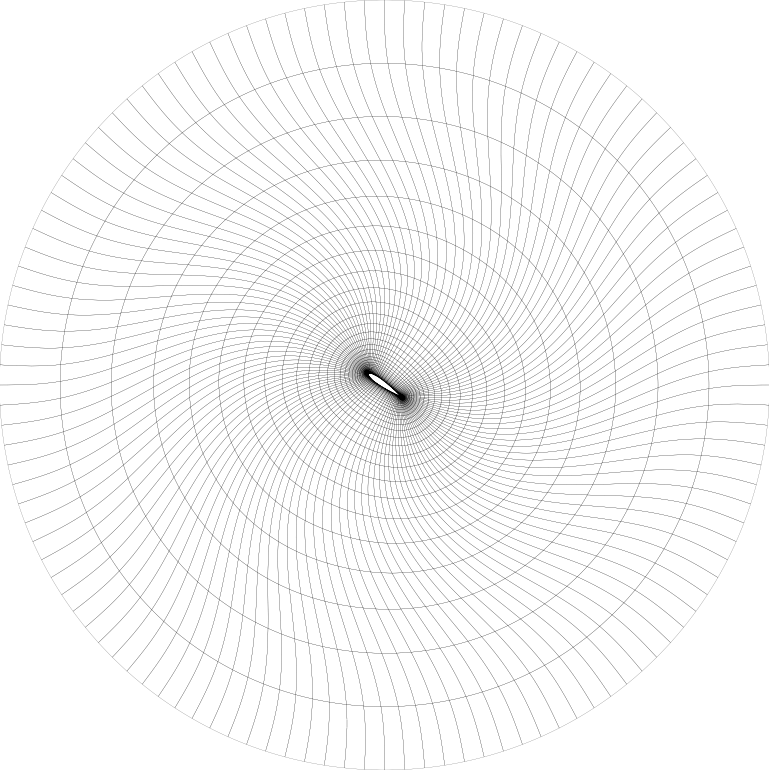
\includegraphics[width=0.4\textwidth]{figs/domain}
  \end{center}
  \caption{
    NACA0015 Airfoil: (Left) Sketch of the airfoil flow problem and its parameters. Solid
    lines indicate Dirichlet boundaries, and dotted lines indicate Neumann
    boundaries. (Right) Sample domain with $\varphi = -\nicefrac{\pi}{4}$.
  }
  \label{fig:airfoil-sketch}
\end{figure}

Two discretizations were compared: a conventional Taylor-Hood method
with quadratic velocities and linear pressures, and a
divergence-conforming discretization with mixed quadratic-linear
velocities and linear pressures.  The latter method produces strongly
solenoidal reduced velocity basis functions, enabling the
aforementioned solenoidal RBMs. The derivation of affine
representations for this geometry transformation is a nontrivial
matter, out of scope for this paper.  We refer to \cite{Fonn2018fdc}
where this is performed explicitly as a truncated Taylor expansion in
$\varphi$.

For both discretizations, an ensemble of $225$ snapshot solutions were
generated on the $15 \times 15$ Gauss quadrature points in the
parameter domain $\mathcal{P}$.  RBMs were then generated with
$m = 10, 20, 30, 40, 50$ basis functions for each of the reduced
bases, giving a total of $m = 30, \ldots, 150$ degrees of freedom in
total. The performance of the two discretizations was evaluated on a
set of $15 \times 15$ \emph{uniformly spaced} points in the parameter
space, chosen so as to avoid the parameter values used to generate the
ensemble.

For evaluating an RBM, the principal quantity of choice is the
\emph{mean relative error}, defined as the mean expected relative
error between the high-fidelity solution and the reduced solution, as
taken over a suitably dense sampling of the parameter space.

Figure~\ref{fig:perf3} shows the true mean relative error as a
function of online solver time.  This reveals the
divergence-conforming (solenoidal) reduced basis method to be
significantly faster for comparable accuracy, because it allows a
velocity and a pressure solution to be found through one $m \times m$
linear system each, rather than a full $3m \times 3m$ linear system as
with conventional methods.  At an error level of roughly $1\%$ the
solenoidal RBMs are already faster by a factor of about $10$, which
can be extremely valuable in the time-sensitive online stage.

Finally, Table~\ref{tbl:airfoil} shows the mean wall-time taken for a
high-fidelity or reduced solution for both methods.  This again
highlights the significant speed improvements achievable with ROMs,
but also how quickly they can deteriorate as the reduced basis grows.
The divergence-conforming method scales much better in terms of
reduced degrees-of-freedom.

\begin{figure}
  \begin{tikzpicture}
    \begin{axis}[
      xlabel={Time (seconds)},
      ylabel={Mean relative error},
      ymode=log,
      xmode=log,
      width=0.9\textwidth,
      height=0.5\textwidth,
      grid=both,
      axis lines=left,
      legend style={
        at={(0.5, -0.2)},
        anchor=north,
        draw=none,
      },
      legend cell align=left,
      legend columns=2,
      ]
      \addplot[blue, thick, mark=*, mark options={solid}]
      table[x index={15}, y index={4}]{data/airfoil-results-no-piola-sups-no-block.csv};
      \addplot[blue, thick, densely dashed, mark=o, mark options={solid}]
      table[x index={15}, y index={8}]{data/airfoil-results-no-piola-sups-no-block.csv};
      \addplot[red, thick, mark=*, mark options={solid}]
      table[x index={11}, y index={4}]{data/airfoil-results-piola-sups-block.csv};
      \addplot[red, thick, densely dashed, mark=o, mark options={solid}]
      table[x index={11}, y index={8}]{data/airfoil-results-piola-sups-block.csv};
      \legend{
        Taylor-Hood ($v$),
        Taylor-Hood ($p$),
        Divergence-conforming ($v$),
        Divergence-conforming ($p$),
      }
    \end{axis}
  \end{tikzpicture}
  \caption{
    NACA0015 Airfoil: Measured mean relative error as a function of
    mean time usage (in seconds), for velocity ($H^1$-seminorm) and
    pressure ($L^2$-norm).  The markers correspond to
    $m=10,20,30,40,50$ degrees of freedom in velocity and pressure
    separately. The time reported includes both the velocity solution
    and the pressure recovery or reconstruction, as appropriate.
    At an error level of $\sim 1 \%$ the solenoidal method has a
    speedup factor of $\sim 10 \times$.
    Bottom left is better.
  }
  \label{fig:perf3}
\end{figure}

\begin{table}
  \begin{center}
    \bgroup\def\arraystretch{1.2}
    \begin{tabular}{rrrrr}
      & \multicolumn{2}{c}{\bf Taylor-Hood} & \multicolumn{2}{c}{\bf Conforming} \\
      \hline
      & Time & Speedup & Time & Speedup \\
      \hline
      Hi-Fi & $\SI{39}{\second}$ & & $\SI{110}{\second}$ & \\
      $m=10$ & $\SI{16}{\milli\second}$ & $2400$ & $\SI{10}{\milli\second}$ & $11000$ \\
      $m=20$ & $\SI{79}{\milli\second}$ & $490$ & $\SI{17}{\milli\second}$ & $6500$ \\
      $m=30$ & $\SI{290}{\milli\second}$ & $130$ & $\SI{32}{\milli\second}$ & $3400$ \\
      $m=40$ & $\SI{750}{\milli\second}$ & $52$ & $\SI{61}{\milli\second}$ & $1800$ \\
      $m=50$ & $\SI{1.6}{\second}$ & $24$ & $\SI{100}{\milli\second}$ & $1100$ \\
      \hline
    \end{tabular}
    \egroup
  \end{center}
  \caption{
    NACA0015 Airfoil: Mean timings and speedup factors for the
    Taylor-Hood and the divergence-conforming methods for different
    numbers of reduced degrees-of-freedom.
  }
  \label{tbl:airfoil}
\end{table}

\section{Numerical example: Transient 2D flow around a cylinder}

The purpose of this section is to argue for the viability of limited
reduced bases for non-stationary flow problems.  The model problem is
flow around a cylinder at $\text{Re} = 100$ without any
parameter-dependence other than time. This is a setup that is known to
produce \emph{vortex shedding}, as seen in Figure~\ref{fig:vortices}.

\begin{figure}
  \begin{center}
    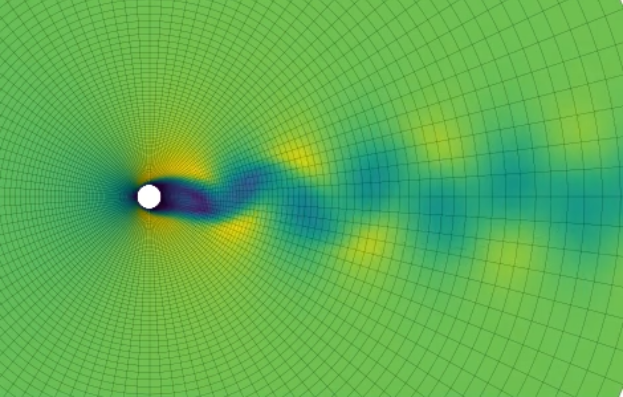
\includegraphics[width=0.48\textwidth]{figs/vortices-hi}
    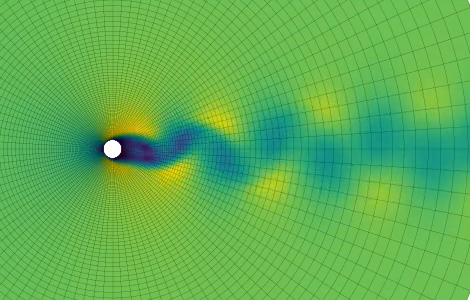
\includegraphics[width=0.48\textwidth]{figs/vortices-lo}
  \end{center}
  \caption{
    2D cylinder flow: Vortex shedding in the wake of the cylinder at
    $\text{Re} = 100$. High-fidelity solution on the left, and an RBM
    with $m=10$ degrees of freedom on the right. The coloring is
    according to flow speed magnitude.
  }
  \label{fig:vortices}
\end{figure}

Typically it takes several timesteps before a simulation reaches the
stage where vortex shedding occurs continuously without significant
variation over time scales other than the primary shedding frequency.
We call this the \emph{terminal stage}, and we propose that this is
the stage of primary interest in many ROM applications.  For example,
in optimal design applications, one is generally interested in
optimizing for the long term behaviour of a system. In contrast, the
time steps before reaching the terminal stage, which we shall call the
\emph{initial stage}, are often of limited interest.

When designing an RBM for a non-stationary problem it is necessary
that the reduced basis provides sufficient approximative power in
every stage.  If the solution at the end of the intial stage is poor,
it is natural to imagine that no value can be found in the solution
for the terminal stage.  One would conclude, therefore, that a
successful reduced basis must account for degrees-of-freedom from both
stages. In this case, however, the vortex shedding behaviour develops
naturally from almost any initial condition.  We argue that, in the
application context previously introduced, if an RBM can reach the
terminal stage in any state whatsoever from which vortex shedding can
develop, such a method is equally as powerful as an RBM with full
approximative power for every stage.

In the following example, we performed a high-fidelity simulation
around a cylinder of radius~$\SI{1}{\meter}$ with an inflow velocity
of $u_\infty = \SI{1}{\meter/\second}$ at timesteps of
$\Delta t = \SI{0.5}{\second}$.  The viscosity was fixed at
$\nu = \SI[parse-numbers=false]{\nicefrac{1}{100}}{\meter^2/\second}$
giving a Reynolds number of $\text{Re} = 100$.  After vortex shedding
stabilized, we collected~$500$ snapshots.  Thus, no snapshots were
collected from the initial stage.

Figure~\ref{fig:initial} shows the behaviour of the drag force on the
cylinder from four reduced models compared to the high-fidelity
method.  We can see that the RBMs behave very differently in the
initial stage, and remain there for many more timesteps, but that they
all reach the terminal stage in due time, and that the drag force as
reported by the reduced methods correspond well to that reported by
the high-fidelity method.

The timing results for this example are comparable to those in
Table~\ref{tbl:airfoil} per timestep, with the caveat that the RBMs
take $4$--$6 \times$ as many timesteps to reach the terminal stage.
The practical speedup factors are therefore about $600$ for the
Taylor-Hood method, and $2800$ for the divergence-conforming method at
$m=10$.  For higher numbers of degrees-of-freedom, the deterioration
accelerates because of the tendency for larger RBMs to take longer to
reach the terminal stage, as seen in Figure~\ref{fig:initial}.  It is
therefore of particular importance that the divergence-conforming
method has good performance characteristics for large~$m$.  It is also
possible to use a smaller RBM for the initial stage, only expanding
the solution space once the terminal stage is reached.  Since reduced
bases of different orders are nested, such a technique would not be
difficult to implement.

\begin{figure}
  \begin{center}
    \begin{tikzpicture}
      \begin{axis}[
        xlabel={Time},
        ylabel={Drag force},
        xticklabels={,,},
        ymin=0.3, ymax=0.8,
        scaled x ticks=false,
        width=0.9\textwidth,
        height=0.6\textwidth,
        grid=both,
        axis lines=left,
        legend style={
          font=\scriptsize,
          at={(1, 0)},
          anchor=south east,
        },
        ]
        \addplot[black, thin] table[x index={0}, y index={1}]{data/forces-big.csv};
        \addplot[red, thin] table[x expr={\thisrowno{0}*25}, y index={1}]{data/forces-05.csv};
        \addplot[blue, thin] table[x expr={\thisrowno{0}*25}, y index={1}]{data/forces-10.csv};
        \addplot[magenta, thin] table[x expr={\thisrowno{0}*25}, y index={1}]{data/forces-15.csv};
        % \addplot[cyan, thin] table[x expr={\thisrowno{0}*25}, y index={1}]{data/forces-20.csv};
        \draw[densely dotted, thin] (axis cs:0,0.655) -- (axis cs:50000,0.655);
        \draw[densely dotted, thin] (axis cs:0,0.649) -- (axis cs:50000,0.649);
        \legend{Hi-Fi, $m=5$, $m=10$, $m=15$};
      \end{axis}
    \end{tikzpicture}
  \end{center}
  \caption{
    2D cylinder flow: Long-term evolution of the drag force of limited
    RBMs in the intial stage, as compared to the high-fidelity method.
  }
  \label{fig:initial}
\end{figure}

\section{Conclusions}

We have demonstrated a significant advantage to using
divergence-conforming high-fidelity methods to produce solenoidal
reduced basis methods.  The resulting RBMs are considerably faster
($\sim 10 \times $) in the online stage than conventional RBMs with
comparable accuracy ($\sim 1 \%$ relative error).  This is owing to
the ``decoupling'' effect of solenoidal basis functions, allowing
separate solutions for velocity and pressure with two smaller linear
systems, as opposed to a simultaneous larger system for both fields.

We have also shown that limited numbers of basis functions are
suitable for non-stationary applications where the primary interest
lies in the stable long-term behaviour of the system, as opposed to
the intial stages.  Snapshots can be sourced only from the terminal
stage of interest without regard for the initial stages.

\clearpage
\ack

The authors acknowledge the financial support from the Norwegian
Research Council and the industrial partners of OPWIND: Operational
Control for Wind Power Plants~(Grant~No.:~268044/E20).
\texttt{https://www.sintef.no/en/projects/opwind/}

\section*{References}

\bibliography{common/references}
\bibliographystyle{iopart-num}

\end{document}
